\documentclass[11pt]{amsart}
\usepackage{geometry}                % See geometry.pdf to learn the layout options. There are lots.
\geometry{letterpaper}                   % ... or a4paper or a5paper or ... 
%\geometry{landscape}                % Activate for for rotated page geometry
%\usepackage[parfill]{parskip}    % Activate to begin paragraphs with an empty line rather than an indent
\usepackage{graphicx}
\usepackage{amssymb}
\usepackage{epstopdf}
\usepackage{setspace}
\onehalfspacing
\usepackage{amsmath}
\newtheorem{theorem}{Theorem}[section]
\newtheorem{corollary}{Corollary}[theorem]
\newtheorem{lemma}[theorem]{Lemma}
\usepackage{amsthm}
 
\theoremstyle{definition}
\newtheorem{definition}{Definition}[section]
 
\theoremstyle{remark}
\newtheorem*{remark}{Remark}
\DeclareGraphicsRule{.tif}{png}{.png}{`convert #1 `dirname #1`/`basename #1 .tif`.png}

\title{Optimal design for nonlinear models with extension in T-sys}
\author{Yi Hua}
%\date{}                                           % Activate to display a given date or no date

\begin{document}
\maketitle
\section{Model and Approximate Design}
Consider a nonlinear regression model $ E(y) = \eta(x,\theta)$ where a response variable $y$ depends on a single regression variable $x$. Assume $y$'s are independent and follow Bernoulli distribution with mean  $\eta(x,\theta)$. In the design of experiment scenario, the regression variable $x$ corresponds to a design point. The collection of design points and corresponding weights $\xi = \{(x_i,w_i), i=\ldots,N\}$ is called an approximate design.  In many cases, for simplification purposes, $z_i$ as a monotone? continuous function of $x_i$ is considered in design. 

The goal of optimal design is to seek optimal choice of $\xi= \{(z_i,w_i), i=\ldots,N\}$  in terms of characteristic of the empirical fisher information matrix, which can be written as \begin{equation}\label{eq:1}
M(\xi,\theta) = P(\theta)(\sum_{i=1}^Nw_iC(\theta,z_i))(P(\theta)^T)
\end{equation}where \begin{equation}\label{eq:2}
C(\theta,z_i) = \left ( \begin{array}{cccc}
\Psi_{11}(z_i) &&&\\
\Psi_{21}(z_i) &\Psi_{22}(z_i)&&\\
\vdots & \vdots &&\\
\Psi_{p1}(z_i) &\Psi_{p2}(z_i)&\cdots&\Psi_{pp}(z_i)\\
\end{array} \right).\end{equation}
The function $\Psi_{m,n}(\theta,z), m,n=1,\ldots,p$  and and $M(\xi,\theta)$ may depend on $\theta$. We will use $  \Psi_{m,n}(z)$ and $M(\xi)$ for simplicity in notation. In \eqref{eq:1} and \eqref{eq:2}, $C(\theta,z)$ is symmetric and $P(\theta)$ is independent of $x$. Our goal is to find a design $\tilde{\xi} = \{(\tilde{z_i},\tilde{w_i}), i=1,\ldots,n\}$ such that $M(\xi)$ is dominated by $M(\tilde{\xi})$ by Loewner Ordering, which means $ M(\tilde{\xi})-M(\xi)$ is a positive definite matrix.

To achieve this goal, Yang (2009) has introduced a strategy that requires the following equations to hold:
\begin{equation}\label{eq: strategy1}
\sum_{i=1}^{n} w_i \Psi_{lt}(z_i) =\sum_{i=1}^{\tilde{n}} \tilde{w_i} \Psi_{lt}(\tilde{z_i}),\end{equation} for $1\le l\le t \le p$ except for some $l=t $, and, \begin{equation}\label{eq: strategy2}
\sum_{i=1}^{n} w_i \Psi_{ll}(z_i) \le \sum_{i=1}^{\tilde{n}} \tilde{w_i} \Psi_{ll}(\tilde{z_i}), \end{equation} 
Note that $\Psi_{lt}$'s, $1 \le l \le t \le p$ may not be linearly independent. This is a sufficient condition of the inequality in Loewner Ordering.


\section{Methodology and limitations} 

Yang (2010) have elaborated a strategy on finding a design that satisfies \eqref{eq: strategy1} and \eqref{eq: strategy2}. Yang (2012) extended the method and was able to increase the efficiency of the design further. The strategy is as follows. Let $\Psi_1,\ldots, \Psi_{k-1}$ be the maximum set of linearly independent nonconstant terms in $p-p_1$ columns of $C(\theta,z)$. Let the remaining columns of $C(\theta,z)$ \[C(\theta,z) = \left ( \begin{array}{cccc}
\Psi_{11}(z) &&&\\
\Psi_{21}(z) &\Psi_{22}(z)&&\\
\vdots & \vdots &&\\
\Psi_{p1}(z_i) &\Psi_{p2}(z_i)&\cdots&\Psi_{pp}(z_i)\\
\end{array}\right).\]to be denoted as $C_{22}(z)$ $\Psi_k^Q$ is defined as follows. 
\[\Psi_k^Q = Q^TC_{22}(z)Q\] where $Q$ is a nonzero vector of dimension $p_1\times 1$. 
hold for \eqref{eq: strategy1} and $\Psi_{k}$ holds for  \eqref{eq: strategy2}.  Here $\Psi_k$ is one of  $\Psi_{ll}, 1\le l \le p$. Note here that when $p_1=1$, $\Psi_k$ and $Q$ are scalar terms. Let $\Phi_0(z) = 1$. It's straightforward to see that our goal in \eqref{eq: strategy1} and \eqref{eq: strategy2} are now 
\begin{equation} \label{eq: st1}
\sum_{i}w_i\Psi_l(z_i)=\sum_{i}\tilde{w_i}\Psi_l(\tilde{z_i}), l=0,1,\ldots, k-1
\end{equation} and \begin{equation} \label{eq: st2}
\sum_{i}w_i\Psi_k^Q(z_i)<\sum_{i}\tilde{w_i}\Psi_k^Q(\tilde{z_i}) \text{  for every nonzero vector Q}
\end{equation} 
\subsection{The Chebyshev System}
We can see that in \eqref{eq: st1} and \eqref{eq: st2},  there is an equivalent matrix form for some $\epsilon>0$ with respect to a given design $S_1 = \{(z_i, w_i), i=1,..,n\} $, and a target design  $S_2 = \{(\tilde{z}_i, \tilde{w}_i), i=1,..,n\}$
\begin{equation}\label{eq: tsys1}
\left ( \begin{array}{cccc}

\Psi_{0}(\tilde{z}_1) &\Psi_{1}(\tilde{z}_1)&\ldots &\Psi_{k}^Q(\tilde{z}_1)\\
\Psi_{0}(\tilde{z}_2) &\Psi_{1}(\tilde{z}_2)&\ldots &\Psi_{k}^Q(\tilde{z}_2)\\
\vdots & \vdots &&\vdots\\
\Psi_{0}(\tilde{z}_n) &\Psi_{1}(\tilde{z}_n)&\ldots &\Psi_{k}^Q(\tilde{z}_n)\\
\end{array}\right) \left(\begin{array}{c}
  \tilde{w}_1    \\
   \tilde{w}_2    \\
   \vdots\\
    \tilde{w}_k    \\
      
\end{array}\right) = \left(\begin{array}{c}
  m_1    \\
   m_2    \\
   \vdots\\
    m_k+\epsilon    \\
      
\end{array}\right) 
\end{equation} where $m_l = \sum_{i}w_i\Psi_l(z_i)$ for $l=0,1,\ldots,k$ . Our goal is to solve for $\{\tilde{w}_i, i=1,\ldots,n\}$ given $\{\tilde{z}_i, i=1,\ldots,n\}$ and $S_1$. In order to guarantee existence of the solution for all values of $\tilde{z}_i$, the matrix $\left(\Psi_j(\tilde{z}_i)\right)_{i,j}$, $i=1,\ldots,n$,$j=0,...,k$ has to have full rank. This further indicates that any $k+1$ rows of $\left(\Psi_j(\tilde{z}_i)\right)_{i,j}$, $i=1,\ldots,n$,$j=0,...,k$ forms a full rank matrix. Without loss of generality, take \{$\tilde{z}_1 \le \ldots\le\tilde{z}_{k+1} $\} and with a few switches in orders of the $\Psi_l(z), l=0,\ldots, k-1$ function, it requires\[det\left ( \begin{array}{cccc}\label{eq: tdef1}

\Psi_{0}(\tilde{z}_1) &\Psi_{1}(\tilde{z}_1)&\ldots &\Psi_{k}^Q(\tilde{z}_1)\\
\Psi_{0}(\tilde{z}_2) &\Psi_{1}(\tilde{z}_2)&\ldots &\Psi_{k}^Q(\tilde{z}_2)\\
\vdots & \vdots &&\vdots\\
\Psi_{0}(\tilde{z}_{k+1}) &\Psi_{1}(\tilde{z}_{k+1})&\ldots &\Psi_{k}^Q(\tilde{z}_{k+1})\\
\end{array}\right)>0 \] or \[det\left ( \begin{array}{cccc}\label{eq: tdef2}

\Psi_{0}(\tilde{z}_1) &\Psi_{1}(\tilde{z}_1)&\ldots &-\Psi_{k}^Q(\tilde{z}_1)\\
\Psi_{0}(\tilde{z}_2) &\Psi_{1}(\tilde{z}_2)&\ldots &-\Psi_{k}^Q(\tilde{z}_2)\\
\vdots & \vdots &&\vdots\\
\Psi_{0}(\tilde{z}_{k+1}) &\Psi_{1}(\tilde{z}_{k+1})&\ldots &-\Psi_{k}^Q(\tilde{z}_{k+1})\\
\end{array}\right)>0 \] for all $\tilde{z}_i \in [A,B]$. \eqref{eq: tdef1} is the  definition of a Tchebyshev System of $\{\Psi_0(z),\Psi_1(z),\ldots, \Psi_k^Q(z)\}$ on the closed finite interval $[A,B]$ and similarly \eqref{eq: tdef2} is the  definition of a Tchebyshev System of $\{\Psi_0(z),\Psi_1(z),\ldots, -\Psi_k^Q(z)\}$ on the closed finite interval $[A,B]$  \cite{tsys}. 

It's worth mentioning here that by matrix algebra, the sign of the determinant of the matrix is invariant to certain column operations.  We can safely multiply each function in $\{\Psi_0(z),\Psi_1(z),\ldots, \Psi_k^Q(z)\}$ by a function $g(z)$ as long as $g(z)>0$ for all $z\in [A,B]$ and that wouldn't change the sign of the determinant. That being said, $\{\Psi_0(z),\Psi_1(z),\ldots, \Psi_k^Q(z)\}$ is a Chebyshev system if and only if $\{\Psi_0(z)g(z),\Psi_1(z)(g),\ldots, \Psi_k^Q(z)(g)\}$ is a Chebyshev system for some function $g(z)>0$ for all $z\in [A,B]$. Also, if we switch the order of the functions in $\{\Psi_0(z),\Psi_1(z),\ldots, \Psi_k^Q(z)\}$, we are actually changing the order of columns in the matrix, which might result in a change of sign in the permuted sequence. Therefore, we need to be careful with the order of the functions in application. We can also do column addition. This means that we can work instead on linearly independent terms of  $\{\Psi_0(z),\Psi_1(z),\ldots, \Psi_k^Q(z)\}$, which will be easier forms than original.



On the other hand, since our target $S_1$ and $S_2$ are both designs, we have $\sum_i^nw_i = \sum_{i=1}^n\tilde{w}_i=1$. This indicates that one of the $\tilde{w}_i$'s is calculated through the rest. Here we will write $\tilde{w}_k = 1-\sum_{i=0}^n \tilde{w}_i$. Then it's clear to see that, other than the equation \eqref{eq: tsys1}, we also need to secure the following "smaller" equation to have solution
\begin{equation}\label{eq: tsys2}
\left ( \begin{array}{cccc}

\Psi_{0}(\tilde{z}_1) &\Psi_{1}(\tilde{z}_1)&\ldots &\Psi_{k-1}(\tilde{z}_1)\\
\Psi_{0}(\tilde{z}_2) &\Psi_{1}(\tilde{z}_2)&\ldots &\Psi_{k-1}(\tilde{z}_2)\\
\vdots & \vdots &&\vdots\\
\Psi_{0}(\tilde{z}_n) &\Psi_{1}(\tilde{z}_n)&\ldots &\Psi_{k-1}(\tilde{z}_n)\\
\end{array}\right) \left(\begin{array}{c}
  \tilde{w}_1    \\
   \tilde{w}_2    \\
   \vdots\\
    \tilde{w}_{k-1}    \\
      
\end{array}\right) = \left(\begin{array}{c}
  m_1    \\
   m_2    \\
   \vdots\\
    m_{k-1}   \\
      
\end{array}\right) 
\end{equation} where $m_l = \sum_{i}w_i\Psi_l(z_i)$ for $l=0,1,\ldots,k-1$. For solution from both \eqref{eq: tsys1} and \eqref{eq: tsys2} to be consistent, it leads to that $\{\Psi_0(z),\Psi_1(z),\ldots, \Psi_{k-1}(z)\}$ needs to be a Tchebyshev system.

Up to this point, we have arrived at a sufficient condition of  \eqref{eq: st1} and \eqref{eq: st2}, which is one of the following  \begin{enumerate}
    \item\label{3.5}$\{\Psi_0(z),\Psi_1(z),\ldots\} $and  $\{\Psi_0(z),\Psi_1(z),\ldots, \Psi_k^Q(z)\}$ form Chebyshev systems for every nonzero vector $Q$, 
     \item\label{3.6} $\{\Psi_0(z),\Psi_1(z),\ldots\} $and  $\{\Psi_0(z),\Psi_1(z),\ldots, -\Psi_k^Q(z)\}$ form Chebyshev systems for every nonzero vector $Q$
\end{enumerate} 

Yang (2012) provided results on the above condition
\begin{theorem}\label{2012a}
For a regression model with a single regression variable $x$, suppose that the information matrix $C(\theta,z)$ can be written as in \eqref{eq:1} and \eqref{eq:2} for $z\in[A,B]$. Partitioning the information matrix and let $\Psi_1,\ldots,\Psi_{k-1},\Psi^Q_{k}$ be defined as aforementioned. Suppose that either \ref{3.5} or \ref{3.6} holds, then the following complete class results hold:
\begin{enumerate}
    \item [(a)] For $k=2n-1$, if \ref{3.5} holds, the designs with at most $n$ support points, including $B$, form a complete class
    
      \item [(b)] For $k=2n-1$, if \ref{3.6} holds, the designs with at most $n$ support points, including $A$, form a complete class
      \item [(c)] For $k=2n$, if \ref{3.5} holds, the designs with at most $n+1$ support points, including both $A$ and $B$, form a complete class
      \item [(d)] For $k=2n$, if \ref{3.6} holds, the designs with at most $n$ support points form a complete class
    
\end{enumerate}
\end{theorem}

\subsection{The sufficient condition: Result of Yang(2010)}

Now that we have found a sufficient condition for \eqref{eq: st1} and  \eqref{eq: st2}, and a tool \ref{2012a}, we are able to identify the complete class for the designs. However, to prove that a sequence of a function is Chebyshev system is not easy. To do that, Yang (2012) proposed the following tools and developed a sufficient condition.

 Define functions $f_{l,t}, 1\le t \le k$; $t\le l \le k$ as follows
\begin{equation}\label{eq: ff}
f_{l,t}(z) = \left \{ \begin{array}{ll}
\Psi_l'(z), & \text{if } t=1,l=1,...,k-1\\
C'_{22}(z), & \text{if } t=1,l=k\\
(\frac{f_{l,t-1}(z)}{f_{t-1,t_1}(z)})', & \text{if } 2\le t\le k, t\le l \le k.
\end{array}\right.
\end{equation}
and   $F(z) = \prod_{l=1}^k f_{l,l}(z)$. With these definitions, Yang showed that $F(z)$ being positive definite is sufficient condition of \ref{3.5} and  $-F(z)$ being positive definite is sufficient condition of \ref{3.6}. Three assumptions are made through the construction of $f_{l,t}(z)$ and $F(z)$ functions and towards the following results. 

The assumptions:
\begin{enumerate}
\item All functions $\Psi$ in the information matrix $C(\theta,z)$ are at least $k$th order differentiable on $(A,B)$.
\item For $1\le l\le k-1$, the functions $f_{l,l}(z)$ have no roots in $[A,B]$.
\item Either $F(z)$ or $-F(z)$ is positive definite for all $z\in [A,B]$
\end{enumerate} 

The main result of Yang (2012) is as below.

\begin{theorem}\label{2012}
For a regression model with a single regression variable $x$, let $z\in[A,B]$, $C(\theta,z)$, $\Psi_1,\ldots, \Psi_{k-1}$ and $\Psi_k^Q$ defined above. With  $F(z) = \prod_{l=1}^k f_{l,l}(z)$, suppose all assumption satisfied above. Then the following complete class results hold:\begin{enumerate}
\item[(a)] For $k = 2n-1$, if $F(z)>0$, the designs with at most $n$ support points, including B, form a complete class.
\item[(b)] For $k = 2n-1$, if $-F(z)>0$, the designs with at most $n$ support points, including A, form a complete class.
\item[(c)] For $k = 2n$, if $F(z)>0$, the designs with at most $n+1$ support points, including both A and B, form a complete class.
\item[(d)] For $k = 2n$, if $F(z)>0$, the designs with at most $n$ support points form a complete class.
\end{enumerate}
\end{theorem}

 This strategy has been applied to many models when all three assumptions are satisfied. However, there are cases when Assumption (2) and (3) are violated we might run into problems. Take complementary log-log model as an example, which has the model formula $P(y=1|x) = 1-e^{-e^{z}}$, $z\in(-\infty,\infty)$. Following the procedure in \ref{2012}, we have the function sequence \{1,$g(z)$, $zg(z)$,$z^2g(z)$\} ,$g(z)=\frac{e^{2z}}{e^{e^z}-1}$, and checked the assumption. With Mathematica we can find that assumption (2) and (3) are violated at $z=0.4660$ and $z=0.0491$. Specifically, we can apply condition (a) of \ref{2012} when $F(z) >0$ $z\in (-\infty, 0.0491)$ and condition (b) when $F(z)<0$ for $z\in(0.0491, 0.4660)$ and $(0.4660,\infty$ respectively. It follows that we can only obtain the complete class for three intervals respectively, each with 2 support points. However, Biedermann, et al \cite{biedermann2006} showed that the $\Phi_p$-optimal design for complementary log-log model defined on $(-\infty,\infty$ is supported on 2 points. The previous strategy has yet been able to combine the three separate designs. 
 
 Another example of this situation is the 2-paraemter logistic model which has formula $P(y=1|x,\theta) = \eta(x,\theta)= \frac{1}{e^{-\beta(x-\alpha)}+1}$ where we let $z = \beta(x-\alpha) \in (-\infty, \infty)$ . Following the procedures from \eqref{eq:1} and \eqref{eq:2} , the information matrix based on a design $\xi = \{(z_i,w_i), i=1,\ldots,N\}$ will have the following form: \begin{equation}
M(\xi) = \sum_{i=1}^{k} w_i \frac{e^z_i}{(1+e^{z_i})^2}P \left( \begin{array}{cc}
1 & z_i\\
z_i & z_i^2
\end{array} \right) P^T,
\end{equation} where \[P = \left( \begin{array}{cc}
\beta & 0\\
0 & -\frac{1}{\beta}
\end{array} \right).\] \\

Our goal is to find a design $\tilde{\xi} = \{(\tilde{z_i},\tilde{w_i}), i=1,\ldots,n\}$ such that $M(\xi)$ is dominated by $M(\tilde{\xi})$ by Loewner Ordering. Let $\phi(z) = \frac{e^z}{(1+e^{z})^2}$. To achieve this goal, if we could have the off-diagonal terms of both matrices to be equal as follows,
\begin{equation}\label{eq: beta_eq1}
\sum_{i=1}^{N} w_i \phi(z_i) = \sum_{i=1}^{n} \tilde{w_i}  \phi(\tilde{z_i}) ,
\end{equation}
and
\begin{equation}\label{eq: beta_eq2}
\sum_{i=1}^{N} w_i  \phi(z_i)z_i = \sum_{i=1}^{n} \tilde{w_i} \phi(\tilde{z_i}) \tilde{z_i},
\end{equation}
then it is sufficient to show that 
\begin{equation}\label{eq: beta_eq3}
\sum_{i=1}^{N} w_i \phi(z_i)z_i^2 \le \sum_{i=1}^{n} \tilde{w_i}\phi(\tilde{z_i})\tilde{z_i}^2.
\end{equation}.

To find solutions to the equations, direct application of \ref{2012} will also run into problems. Following the procedure of \ref{2012a},we need to show \{$1$ ,$ \phi(z)$, $z\phi(z)$, and $z^2\phi(z)$\} is a Chebyshev System. Also $\phi(z)>0$ holds for all $z$, therefore we can divide each term by $\phi(z)$ and move $1/\phi(z)$ to the last position (the sign changed) without loss of generality. The sequence is then equivalent to $\Psi_0(z) = 1$ , $\Psi_1(z) = z$ , $\Psi_2(z) = z^2$ , $\Psi_3(z) = -1/\phi(z)$. Calculation of $f_{l,l}(z)$, $l=1,2,3$ shows that $f_{1,1}(z) = 1$, $f_{2,2}(z) = 2$, $f_{3,3}(z) = -3 (1 + e^z) + e^{-z} (1 + e^z)^2/2 + 
 3 e^{-z} (2 e^{2 z} + 2 e^z (1 + e^z))/2 - 
 e^{-z} (6 e^{2 z} + 2 e^z (1 + e^z))/2 $.  \[F(z) = -6 (1 + e^z) + e^{-z} (1 + e^z)^2 + 
 3 e^{-z} (2 e^{2 z} + 2 e^z (1 + e^z)) - 
 e^{-z} (6 e^{2 z} + 2 e^z (1 + e^z))\]
 \begin{figure}[h]
     \centering
     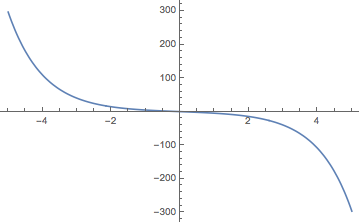
\includegraphics[scale = 0.5]{logistic.png}
     \caption{$F(z)$ for 2-parameter logistic model}
     \label{fig:logistic}
 \end{figure}
 Apparently, third assumption is not satisfied throughout $(-\infty,\infty)$ since $F(0)=0$, but we do get results for $(-\infty,0)$ and $(0,\infty)$ separately. Specifically for $z>0$, $F(z) <0$, and for $z<0$, $F(z) >0$. To get around this hurdle, we could apply \ref{2012} for $z\in[\epsilon, \infty)$ and $z\in(-\infty,-\epsilon]$, $\epsilon>0$,respectively. Here $k=3$. For $z\in[\epsilon, \infty)$, $\epsilon>0$, $F(z)<0$,  designs with 2 support points including $\epsilon$ form a complete class. For $z\in(-\infty,-\epsilon]$, $\epsilon>0$, $F(z)>0$,designs with 2 support points including $-\epsilon$ form a complete class. As $\epsilon\to 0$, the optimal design for each side of $0$ will be \{0,$x_1>0$\} and \{0,$x_2<0$\}. On the other hand Biederman (2006) was able to show that 2- parameter logistic regression defined on $(-\infty,\infty)$ has $\Phi_p$-optimal design with 2 support points.
 
 We try to work with the function sequence \{$1$ ,$\phi(z)$, $z\phi(z)$, and $z^2\phi(z)$\} and insert some ancillary functions. Here we insert $1/(1+e^z)^2$ in front of $1$. We then are actually now working with equations 
 
\begin{equation}\label{eq: log_eq1}
\sum_{i=1}^{N} w_i \frac{1}{(1+e^{z_i})^2} = \sum_{i=1}^{n} \tilde{w_i}  \frac{1}{(1+e^{\tilde{z_i}})^2} ,
\end{equation}

\begin{equation}\label{eq: log_eq2}
\sum_{i=1}^{N} w_i  = \sum_{i=1}^{n} \tilde{w_i}  ,
\end{equation}

\begin{equation}\label{eq: log_eq3}
\sum_{i=1}^{N} w_i \phi(z_i) = \sum_{i=1}^{n} \tilde{w_i}  \phi(\tilde{z_i}) ,
\end{equation}

\begin{equation}\label{eq: log_eq4}
\sum_{i=1}^{N} w_i  \phi(z_i)z_i = \sum_{i=1}^{n} \tilde{w_i} \phi(\tilde{z_i}) \tilde{z_i},
\end{equation}

\begin{equation}\label{eq: log_eq5}
\sum_{i=1}^{N} w_i \phi(z_i)z_i^2 \le \sum_{i=1}^{n} \tilde{w_i}\phi(\tilde{z_i})\tilde{z_i}^2.
\end{equation}.Note here that \ref{eq: log_eq2} is also inherent in \ref{eq: beta_eq1}-\ref{eq: beta_eq3} since $\xi$ and $\tilde{\xi}$ are both designs. Since we now have one extra \ref{eq: log_eq1} in the equation system \ref{eq: log_eq1}-\ref{eq: log_eq5} will have solutions that also satisfy \ref{eq: beta_eq1}-\ref{eq: beta_eq3}, but will most certainly include more $(\tilde{z_i},\tilde{w_i})$. In this sense, the insertion of some  "ancillary" functions will not affect the validity of the solution, although it may most likely include more support points than we desired.

Now that we have a "bigger" design, we'll see how the ancillary functions may help with the violated assumptions. We are now working with \{$1/(1+e^z)^2$, $1$ ,$\phi(z)$, $z\phi(z)$, and $z^2\phi(z)$\}. We can do a similar trick of multiplying each function with $(1+e^z)^2>0$ , take linearly independent terms and check if  \{$1$, $e^{2z}$ ,$e^z$, $ze^z$, $z^2e^z$\} is a Chebyshev system. We then proceed to use \ref{2012} and have $f_{1,1}(z) = 2e^{2z}$, $f_{2,2}(z) = -e^{-z}/2$,$f_{3,3}(z) = 1$,$f_{4,4}(z) = 2$, and $f(z) = -2e^z<0$ for $z\in(-\infty,\infty)$. Now we can safely apply \ref{2012} on $[-A,B]$ for any  $A,B>0$. Luckily, we have that designs with at most 2 support points form a complete class. \\




%  In Yang (2009), the author managed to "combine" optimal designs of the two sides, using the fact that $\phi(z)$ is an even function, and there exist a complete class of 2 support-point design, in which the two point are symmetric about $0$. The author also managed to show the same strategy used in finding design with two symmetric point for 2-parameter probit model. For double exponential and double reciprocal model, the author showed there exist a complete class of 3 support that contains 0 and two symmetric points. All results are based on the symmetry of the above models.
 


We have now seen from the 2-parameter logistic model that use of ancillary functions ($1/(1+e^z)^2)$ helped solve the problem of assumption violation. We now formally introduce the use of ancillary functions for general models. 

 
 
For nonlinear model $E(y) = \eta(x,\theta)$, let $S_1 = \{\Psi_1(z), \ldots,\Psi_{k-1}(z) ,\Psi_k^Q(z)\}$ be functions defined above. Insert $ S_2 =\{\phi^*_1(z), \phi^*_2(z),\ldots, \phi^*_{k_1}(z)\}$ to $S_1$ before  $\Psi_k^Q(z)$. (The order of the terms in $S_1$ remains unchanged). Here $S_2$ are mutually linearly independent and independent of  $S_1$ element-wise. Denote the new sequence as  $S_3 = $\{$\tilde{\Psi}_1(z), \ldots,\tilde{\Psi}_{k+k_1-1}(z)$, $\tilde{\Psi}_{k+k_1}^Q(z)$\}. Let $\tilde{\Psi}_0(z) = 1$. Consider the new sequence $S_3$ as the function sequence used in \eqref{eq: st1} and \eqref{eq: st2}, we will have (ignoring the order) \begin{equation}\label{eq: added1}
\sum_{i}w_i\Psi_l(z_i)=\sum_{i}\tilde{w_i}\Psi_l(\tilde{z_i}), l=0,1,\ldots, k-1    
\end{equation}
\begin{equation}\label{eq: added2}
\sum_{i}w_i\phi_j^*(z_i)=\sum_{i}\tilde{w_i}\phi_j^*(\tilde{z_i}), j=1,\ldots, k_1    
\end{equation}and \begin{equation}\label{eq: added3}
\sum_{i}w_i\Psi_k^Q(z_i)<\sum_{i}\tilde{w_i}\Psi_k^Q(\tilde{z_i}) \text{  for every nonzero vector Q}.
\end{equation} 

Therefore, the function sequence with ancillary functions will still lead to a complete class of designs that is "optimal" in terms of Loewner Ordering. The new design may have to include more support points than desired. However, we'll show in next section that for some models, the "extra" points can actually be removed.

Since all original $\Psi$ functions are from information matrix $C(\theta,z)$, the extended function sequence also suggests an "enlarged" information matrix $\tilde{C}(\theta,z)$. What we do is to add rows and columns to $C(\theta,z)$ and fill in the ancillary function symmetrically. Consider $k_1\le p+1$, we can write \begin{equation}
   \tilde{C}(\theta,z) = \left ( \begin{array}{c|ccccc}
\multicolumn{1}{c}{\phi^*_1}& \ldots& \phi^*_{k_1} &0 &\ldots& 0\\\cline{2-6}
\vdots &  &&&&\\
\phi^*_{k_1} &&&&&\\
0 &\multicolumn{5}{|c}{C(\theta,z)}\\
\vdots &&&&&\\
0&&&&&
\end{array}\right)_{(p+1)\times (p+1)}.
\end{equation} 

When $ p+1< k_1 \le2p+3$, we can write\begin{equation}
   \tilde{C}(\theta,z) = \left ( \begin{array}{cc|ccccc}
\phi^*_{p+2}& \multicolumn{1}{c}{\phi^*_{p+3}}&  \ldots& \phi^*_{k_1} &0 &\ldots& 0\\
\phi^*_{p+3}&\multicolumn{1}{c}{\phi^*_{1}}& && \ldots&& \phi^*_{p+1}\\\cline{3-7}
\vdots &  &&&&&\\
\phi^*_{k_1} &&&&&\\
0 &\vdots &\multicolumn{5}{|c}{C(\theta,z)}\\
\vdots &&&&&&\\
0&\phi^*_{p+1}&&&&&
\end{array}\right)_{(p+2)\times (p+2)}.
\end{equation} We can write $\tilde{C}(\theta,z)$ for larger $k_1$ following the same procedure if needed. However, since our goal is to obtain a design with minimal support, we usually expect $k_1$ to be small. We will discuss the details in next section. $\tilde{C}(\theta,z)$ will be the surrogate of $C(\theta,z)$ to apply \ref{2012}.



%\begin{theorem}(show that ancillary terms doesn't change inequality and how many more support points will be added according to the number of ancillary functions added)
%For nonlinear model $E(y) = \eta(x,\theta)$, let $\Psi_1, \ldots,\Psi_{k-1}$ and $\Psi_k^Q(z)$ be functions defined above. Add $\phi^*_1(z), \phi^*_2(z),\ldots, \phi^*_{k_1}(z)$ to the function sequence before  $\Psi_k^Q(z)$. Here  $\phi^*_1(z), \phi^*_2(z),\ldots, \phi^*_{k_1}(z)$ are mutually linearly independent and independent of   $\Psi_1, \ldots,\Psi_{k-1}$ and $\Psi_k^Q(z)$ (element-wise). Denote the new sequence as  \{$\tilde{\Psi_1}, \ldots,\tilde{\phi}_{k+k_1-1}, \tilde{\phi}_{k+k_1}^Q(z)$\}. Let $\tilde{\phi}_0(z) = 1$. \\

%If we have \begin{equation}\label{cheby+}\{\tilde{\phi}_0(z), \tilde{\phi}_1(z), \ldots,\tilde{\phi}_{k+k_1-1}(z)\}  \text{ and }  \{\tilde{\phi}_0(z), \tilde{\phi}_1(z), \ldots,\tilde{\phi}_{k+k_1-1}(z), \tilde{\phi}_{k+k_1}^Q(z)\}  \end{equation} form Chebyshev systems for every nonzero vector $Q$ or \begin{equation}\label{cheby-} \{\tilde{\phi}_0(z), \tilde{\phi}_1(z), \ldots,\tilde{\phi}_{k+k_1-1}(z)\}  \text{ and }   \{\tilde{\phi}_0(z), \tilde{\phi}_1(z), \ldots,\tilde{\phi}_{k+k_1-1}(z), -\tilde{\phi}_{k+k_1}^Q(z)\}  \end{equation}form Chebyshev systems for every nonzero vector $Q$.\\	\end{theorem}

 

%  The expanded $C(\theta,z)$ will be \[ \tilde{C}^*(\theta,z) = \phi(z)\left(\begin{array}{ccc}
% 1 &e^{2z}&0\\
% e^{2z}&e^z & ze^z\\
% 0& ze^z & z^2e^z
% \end{array} \right).\]Note now $k=4$. Calculate $f_{l,l}(z), l=1,\ldots, 4$, we have $f_{1,1}(z) = 2e^{2z}$, $f_{2,2}(z) = -e^{-z}/2$ , $f_{3,3}(z) = 1$, $f_{4,4}(z) = 2$. As s result $F(z)<0$ for $z\in (-\infty, \infty)$. We have condition (d) satisfied and the designs with at most 2 support points form a complete class. This result is consistent with the conclusion in Yang (2009). \\
 



\section{Main Results}
% We have shown in the 2-parameter logistic model that our strategy are able to deal with the failed assumptions. Before getting to the details of ancillary functions, we will justify the extension to models defined on open interval first. In Yang (2010) and Yang 2012), the results all focused on models defined on closed intervals. The following result shows that we will not have issue of "non-informative " support points with models defined on closed interval. This is not the case when extended to open intervals. 

% \begin{lemma}(Models defined on $[A,B]$ cannot have an optimal design that includes support point $I(A)$ or $I(B) =0$)

% Suppose we have a nonlinear regression model that is defined on $[A,B]$. Information matrix are defined as \eqref{eq:1} and \eqref{eq:2}. Suppose there exist $z^*\in [A,B]$ such that $I(z^*)=0$, the optimal design decided by Loewner ordering will not include that point.
% \end{lemma}
 We have seen in previous sections of how ancillary functions can help solve the violated assumptions of \ref{2012}. We also pointed out that use of ancillary functions as a solution may result in more support points than desired. We would like to show in the following results that, for some functions defined on open interval, the added support points could be removed from the design and we will still ultimately have a design with minimal support. 
 
Since our previous strategy tends to provide optimal design class that includes one or two boundary points, we use following definition to classify 4 types of models in terms of their properties on the boundary points. 
\begin{definition} We categorize models defined on $(A,B)$ into the following 4 types\begin{enumerate}
    \item Type I: $\lim_{z\to A}I(z)=0$ and $\lim_{z\to B}I(z)\ne 0$
    \item Type II: $\lim_{z\to A}I(z)\ne 0$ and $\lim_{z\to B}I(z)=0$
    \item Type III: $\lim_{z\to A}I(z)= 0$ and $\lim_{z\to B}I(z)=0$
    \item Type IV: $\lim_{z\to A}I(z)\ne 0$ and $\lim_{z\to B}I(z)\ne0$
\end{enumerate}
\end{definition}

% \begin{lemma} For nonlinear models with response $E(Y) = \eta(\theta,z)$, $z\in (A,B)$. If there exist $z^*\in [A,B]$ such that \[\lim_{z\to z^*}(\frac{\partial\eta(\theta,z)}{\partial \theta}) = 0\]
% then $\lim_{z\to z^*}I(\theta,z)=0$
% \begin{proof}
% Binary response
% \[\lim_{z\to z^*}I(\theta,z) = \lim_{z\to z^*}\frac{(\frac{\partial\eta(\theta,z)}{\partial \theta})(\frac{\partial\eta(\theta,z)}{\partial \theta})^T}{\eta(\theta,z)(1-\eta(\theta,z))} = 0\]


% %  Continuous response
% %  \[\lim_{z\to z^*}I(\theta,z) = \lim_{z\to z^*}(\frac{\partial\eta(\theta,z)}{\partial \theta})(\frac{\partial\eta(\theta,z)}{\partial \theta})^T = 0\]
%  \end{proof}
%  \end{lemma}

\begin{lemma}\label{removepts}
 For a regression model with a single regression variable $z$ defined on $(A,B)$. Consider subset $[A^*,B^*]\subset (A,B)$ , on which we form a complete class of design with \ref{2012} denoted by $S_1$ = \{$(z_1,w_1)$,$(z_2,w_2)$,$\ldots$, $(z_n,w_n)$\} where $A^*\le z_1,\le \ldots,\le z_n\le B^*$, then\begin{enumerate}
     
     \item If the model is of Type I , and $z_1=A^*$,then $S_1$ is dominated by \{$(z_2,w_1+w_2)$,$\ldots$, $(z_n,w_n)$\} where $A^*<z_2 \le,\ldots,\le z_n\le B^*$
     \item If the model is of Type II , and $z_n=B^*$,then $S_1$ is dominated by \{$(z_1,w_1+w_n)$,$\ldots$, $(z_{n-1},w_{n-1})$\} where $A^*\le z_1 \le,\ldots,\le z_{n-1}< B^*$
     \item If the model is of Type III , and $z_n=B^*$,then $S_1$ is dominated by a design with no support on $A^*$ or $B^*$.
     \item In all other cases, no support points will be removed from $S_1$.
 \end{enumerate}
\end{lemma}

From \ref{removepts}, we can see that it is possible for us to reduce the support for certain types of model. With this tool, the enlarged design with ancillary functions may be reduced back to minimal support. 

  

 

% We now are able to extend the conclusion in \ref{2012} to models defined on open interval $(A,B)$ under following assumptions. \begin{enumerate}
% \item All functions $\Psi$ in the information matrix $C(\theta,z)$ are at least $k$th order differentiable on $(A,B)$.
% \item For $1\le l\le k-1$, the functions $f_{l,l}(z)$ have no roots in $(A,B)$.
% \end{enumerate} 


% \begin{theorem}\label{2012open}
% For a regression model with a single regression variable $x$, let $z\in(A,B)$, $C(\theta,z)$, $\Psi_1,\ldots, \Psi_{k-1}$ and $\Psi_k^Q$ defined above. With  $F(z) = \prod_{l=1}^k f_{l,l}(z)$, suppose that either $F(z)$ or $-F(z)$ is positive definite for all $z\in (A,B)$. Then the following complete class results hold:\begin{enumerate}
% \item[(a)] For $k= 2n-1$, if Type II or Type III models have $F(z)>0$,  designs with at most $n-1$ support points form a complete class; if Type I or Type IV models have $F(z)>0$,  designs with at most $n$ support points form a complete class. 
% \item[(b)] For $k= 2n-1$, if Type I or Type III models have $-F(z)>0$,  designs with at most $n-1$ support points form a complete class; if Type II or Type IV models have $-F(z)>0$,  designs with at most $n$ support points form a complete class. 
% \item[(c)] For $k = 2n$, if Type III model have $F(z)>0$, designs with at most $n-1$ support points form a complete class; if Type I or Type II model have $F(z)>0$, designs with at most $n$ support points form a complete class; if Type IV model have $F(z)>0$, designs with at most $n+1$ support points form a complete class
% \item[(d)] For $k = 2n$, if models of any type have $-F(z)>0$, designs with at most $n$ support points form a complete class.
% \end{enumerate}
% \end{theorem}
% \begin{proof} 
% The proof is similar for the four conditions. We will here show for (a)  \\
% By \ref{2012}, if $k = 2n-1$ and $F(z)>0$, design with at most n support points form a complete class. Consider for any design $\xi = \{z_1,z_2,\ldots, z_n\}$, there exist $\tilde{\xi} = \{\tilde{z}_1,\tilde{z}_2,\ldots, \tilde{z}_{n-1}, B-\epsilon\}$, $\epsilon>0$ such that \[M(\xi)\le M(\tilde{\xi}) =\sum_i^{n-1} \tilde{w}_iI(\tilde{z}_i)+\tilde{w}_nI(B-\epsilon) \] 
% Since for Type II or Type III models,  $\lim_{z\to B}I(z)=0$, we have zero information at $B$. Without loss of generality, we could assign $w_n$ to $\tilde{z_1}$, which lead to a design $\{(\tilde{z}_1, \tilde{w}_1+\tilde{w}_n), (\tilde{z}_2, \tilde{w}_2),\ldots,(\tilde{z}_{n-1}, \tilde{w}_{n-1}) \}$. This design has $n-1$ support points. 
% For Type II or Type III models, $\lim_{z\to B}I(z)\ne0$ so we are not able to eliminate this point from design. The design with $n$ support points form a complete class.
% \end{proof}




% With \ref{2012open}, we are able to deal with models defined on open interval and eliminate the boundary points that provide 0 information asymptotically. \\

% The next issue to address is the resolution to failed assumptions. In the example of 2-parameter logistic model, the ancillary function enables us to use \ref{2012} with minimal support. In many other cases, the aid of ancillary functions will work at the price of getting a design with more support points. Below is an tentative strategy of choosing ancillary function  %The validity of ancillary functions is also shown. Suppose we already have the ancillary functions and $\tilde{F}(z)>0$ or $-\tilde{F}(z)>0$ 
The following is a tentative procedure of which may be helpful for finding the ancillary functions. We'll demonstrate with examples of how this procedure is used in next section.

\begin{theorem}\label{proc}(How to insert ancillary functions: still working)
Given a nonlinear model, suppose for a function sequence $S_1 = \{\Psi_l(z), l = 1,\ldots,k\}$, neither $F(z)$ or $-F(z)$ is positive definite, we can use the following steps to insert ancillary functions to the sequence. Let $S = S_1$.
\begin{enumerate}
    \item Select a function $\phi(z)$ that is the common factor of most $\Psi$ functions. Choose another one if it is linearly dependent to functions in $S$. If $1\not\in S$, let $\phi(z) = 1$. Update $S = S\cup\{\phi(z)\}$. Update $\tilde{C}(\theta,z)$ with $S$.
    \item Multiply each term of $S$ by least common multiples of the denominators, if any. Update $\tilde{C}(\theta,z)$ 
    \item Take Minimal common factors of the sequence. Start from adding factors shared among most $\Psi$ functions. It will , after matrix algebra, be placed before the lowest order term that contains that factor. Check $F(z)$, if not satisfying the assumptions continue until run out of factors.
    
    \item Clean up the functions so that they are linearly independent, leaving the terms of highest order as is. Update $S = {S,\phi(z)}$. Update $\tilde{C}(\theta,z)$ with $S$.
     \item Calculate $\tilde{F}(z)$. Check if $\tilde{F}(z)$ or $-\tilde{F}(z)$ is positive definite. Record $k_1$ as the number of functions added. If not, repeat 1-3.
\end{enumerate}
\end{theorem}

% \begin{theorem}(how many ancillary functions to use/ where to insert)For a given model with predictor variable $z$ and information matrix at a point $z$ $I(z)$, $z\in[A,B]$, suppose the assumption of \ref{2012} is violated for a function sequence $\{\Psi_0(z),\Psi_1(z),\ldots, \Psi_k(z)\}$, we can insert $k_1$ ancillary functions into the sequence so that the number of support point remain the same. The strategy is as follows, \begin{enumerate}
%     \item If $\lim_{z\to A}I(z)=0$, choose $k_1\le 3$ such that $k+k_1 = 2n-1$ , change the position of insertion so that $-F(z)>0$ for all $z\in [A,B]$.
%     \item If $\lim_{z\to B}I(z)=0$, choose $k_1\le 3$ such that $k+k_1 = 2n-1$ , change the position of insertion so that $F(z)>0$ for all $z\in [A,B]$.
%     \item If $\lim_{z\to A}I(z)=0$ and $\lim_{z\to B}I(z)=0$ , choose $k_1\le 3$ such that $k+k_1 = 2n$, change the position of insertion so that $F(z)>0$ for all $z\in [A,B]$.
%     \item If $\lim_{z\to A}I(z)\ne 0$ and $\lim_{z\to B}I(z)\ne 0$ , choose $k_1\le 3$ such that $k+k_1 = 2n$, change the position of insertion so that $-F(z)>0$ for all $z\in [A,B]$.
% \end{enumerate}

% \end{theorem}



% \begin{corollary}(Closed interval, assumptions failed)
% For a regression model with a single regression variable $x$, let  $z\in[A,B]$, $C(\theta,z)$, $\Psi_1(z), \ldots,\Psi_{k-1}(z)$ and $\Psi_k^Q(z)$ be as in \ref{2012}. Assume all functions $\Psi_i(z)$, $i=1,..,k$ are at least $k$th order differentiable on $(A,B)$ element-wise. Also assume there exist at least one $l_0$, $1\le l_0\le k-1$, and $z^*\in [A,B]$, such that $f_{l_0,l_0}(z^*) = 0 $. Use $k_1$ ancillary functions to extend the function sequence to \{$\tilde{\Psi}_1(z), \ldots,\tilde{\Psi}_{k+k_1-1}(z), \tilde{\Psi}_{k+k_1}^Q(z)$\} as in \ref{proc}. Assume $\tilde{F}(z) = \prod_{l=1}^{k_1+k}\tilde{f}_{l,l}(z)$ with the new sequence. Suppose that either $\tilde{F}(z)$ or $-\tilde{F}(z)$ is positive definite for all $z\in [A,B]$. The following complete class results hold \begin{enumerate}
% \item[(a)] For $k+k_1= 2n-1$, if $\tilde{F}(z)>0$,  designs with at most $n$ support points, including B, form a complete class. 
% \item[(b)] For $k+k_1= 2n-1$, if $-\tilde{F}(z)>0$,  designs with at most $n$ support points, including A, form a complete class.
% \item[(c)] For $k+k_1 = 2n$, if $\tilde{F}(z)>0$,  designs with at most $n+1$ support points, including A and B, form a complete class.
% \item[(d)] For $k+k_1 = 2n$, if $-\tilde{F}(z)>0$,  designs with at most $n$ support points form a complete class.

% \end{enumerate} 

% \end{corollary}


% Through above results, we can see that, nonlinear models that failed assumptions can use ancillary functions to find optimal design at the cost of including extra support on the boundary. Among these models, Type I, II and III models under certain conditions may enable us to remove the extra support points and achieve minimal support. We will demonstrate the combination of two main results in the next section.




\section{More examples}

 \subsection{Beta-Poisson model}

In  studies of binary dose response model, Beta-Poisson model is an important model \cite{haas1983}. The response $y$ follows a Bernoulli distribution with the expected success probability of the following form
\[
P(y=1|x,\theta) = \eta(x,\theta)= 1-(1+\frac{x}{\theta_2})^{-\theta_1}.
\]
 Here $x> 0$ is dose level, with $\theta_1>0$ being the infectivity and $\theta_2>0$ being the shape parameter. Let $z = log(1+\frac{x}{\theta_2})$, and we know $z>0$. Consider range of $z$ to be $[\epsilon,+\infty)$ for $\epsilon>0$. Simple calculation shows that it is a Type I model. The information matrix based on a design $\xi = \{(z_i,w_i), i=1,\ldots,N\}$ will have the following form: \begin{equation}
M(\xi) = \sum_{i=1}^{k} w_iP C(\theta,z_i)P^T,C(\theta,z_i) = \frac{e^{-\theta_1z_i}}{1-e^{-\theta_1z_i}}\left( \begin{array}{cc}
z_i^2 & z_i(1-e^{-z_i})\\
z_i(1-e^{-z_i}) & (1-e^{-z_i})^2
\end{array} \right) 
\end{equation} where \[P = \left( \begin{array}{cc}
1 & 0\\
0 & -\frac{\theta_1}{\theta_2}
\end{array} \right).\] 

Our goal is to find a design $\tilde{\xi} = \{(\tilde{z_i},\tilde{w_i}), i=1,\ldots,n\}$ such that $M(\xi)$ is dominated by $M(\tilde{\xi})$ by Loewner Ordering, which means \[det(M(\tilde{\xi})-M(\xi))>0.\] Let $\phi(z) = \frac{e^{-\theta_1z}}{1-e^{-\theta_1z}}$. To achieve this goal, if we could have the off-diagonal terms of both matrices to be equal as follows,
\begin{equation}\label{eq: beta2_eq1}
\sum_{i=1}^{N} w_i \phi(z_i)z_i(1-e^{-z_i}) = \sum_{i=1}^{n} \tilde{w_i}  \phi(\tilde{z_i}) \tilde{z_i}(1-e^{-\tilde{z_i}}),
\end{equation}
then it is sufficient to show that 
\begin{equation}\label{eq: beta2_eq2}
\sum_{i=1}^{N} w_i  \phi(z_i)(1-e^{-z_i})^2 \le \sum_{i=1}^{n} \tilde{w_i} \phi(\tilde{z_i}) (1-e^{-\tilde{z_i}})^2,
\end{equation}
and
\begin{equation}\label{eq: beta2_eq3}
\sum_{i=1}^{N} w_i \phi(z_i)z_i^2 \le \sum_{i=1}^{n} \tilde{w_i}\phi(\tilde{z_i})\tilde{z_i}^2.
\end{equation} where equality in \eqref{eq: beta2_eq2} and \eqref{eq: beta2_eq3} cannot be equal at the same time.\\

Since we only have 3 unique terms in $M(\xi)$, let $\Psi_0(z) = 1$ , $\Psi_1(z) = z(1-e^{-z})\phi(z)$ , $\Psi_2(z) = (1-e^{-z})^2\phi(z)$ , $\Psi_3(z) = z^2\phi(z)$. Calculation of $f_{l,l}$, $l=1,2,3$ become too complicated due to the additive terms in $\Psi$ functions. Using Mathematica, we can also see that for $\theta_1>0$, second assumption is not satisfied for $z>0$ and the $f_{l,l}$, $l=1,2,3$ have at least one root for $\theta_1$. Although the fact that some $\Psi$ functions are additive is not the reason why the method doesn't work, it motivates us to try "separating" the terms through adding ancillary terms.  We then can solve the problem as if we had a larger information matrix to start with. 

Note that $\phi(z)(1-e^{-z})^2 = \phi(z)(1+e^{-2z}-2e^{-z}) = \phi(z)+\phi(z)e^{-2z}-2\phi(z)e^{-z}$. In order to show Equation \eqref{eq: beta2_eq2}, it is sufficient to show 
\begin{equation}\label{eq: beta_eq21}
\sum_{i=1}^{k} w_i \phi(z_i) = \sum_{i=1}^{k} \tilde{w_i}  \phi(\tilde{z_i}),\end{equation}
\begin{equation}\label{eq: beta_eq22}
-\sum_{i=1}^{k}2 w_i  \phi(z_i)e^{-z_i} = -\sum_{i=1}^{k}2 \tilde{w_i} \phi(\tilde{z_i}) e^{-\tilde{z_i}},
\end{equation}
and
\begin{equation}\label{eq: beta_eq23}
\sum_{i=1}^{k} w_i \phi(z_i)e^{-2z_i} < \sum_{i=1}^{k} \tilde{w_i}\phi(\tilde{z_i})e^{-2\tilde{z_i}}
\end{equation}

Similarly for Equation \eqref{eq: beta2_eq1},since  $\phi(z)(1-e^{-z}) = \phi(z)z-\phi(z)ze^{-z}$, it is equivalent to show 
\begin{equation}\label{eq: beta_eq11}
\sum_{i=1}^{k} w_i \phi(z_i)z_i = \sum_{i=1}^{k} \tilde{w_i}  \phi(\tilde{z_i})\tilde{z_i},\end{equation} 
and  
\begin{equation}\label{eq: beta_eq12}
-\sum_{i=1}^{k} w_i  \phi(z_i)e^{-z_i} = -\sum_{i=1}^{k} \tilde{w_i} \phi(\tilde{z_i}) e^{-\tilde{z_i}}.\end{equation} 
Note here that Equation \eqref{eq: beta_eq12} is equivalent to Equation  \eqref{eq: beta_eq22}.  Our problem is transformed into a sufficient condition that Equation \eqref{eq: beta_eq21} -\eqref{eq: beta_eq11} all hold. The complicated elements of $M(\xi)$ is split into functions of simple forms. \\

The linearly independent terms of the above equations are $\phi(z), z\phi(z), \phi(z)e^{-z}$, $\phi(z)ze^{-z}$, $z^2\phi(z)$ and $ \phi(z)e^{-2z}$. We need to point out that although we have initiated the process as a ?separation? of the additive terms, it is actually fulfilled by adding 1, $\phi(z)z$,$\phi(z)$ and  $\phi(z)e^{-z}$ to the sequence \{$z^2\phi(z)$, $z(1-e^{-z})\phi(z)$, $(1-e^{-z})^2\phi(z)$ \},  and take linearly independent terms. Note here information matrix is "expanded" as
\begin{equation}
   \tilde{C}(\theta,z) = \left ( \begin{array}{cc|cc}
1& \multicolumn{1}{c}{0}&  0&  0\\
0&\multicolumn{1}{c}{\phi(z)}&z\phi(z)&  e^{-z}\phi(z)\\\cline{3-4}
0&z\phi(z) & & \\
0&e^{-z}\phi(z) &\multicolumn{2}{|c}{C(\theta,z)}
\end{array}\right).
\end{equation}

where\[ C(\theta,z) = \phi(z)\left(\begin{array}{cc}
z^2 & z(1-e^{-z})\\
z(1-e^{-z}) & (1-e^{-z})^2
\end{array} \right).\] Since $\phi(z)>0$, we can divide all the terms by $\phi(z)$. After taking the linearly independent terms, we are now working on an equivalent information matrix\[ \tilde{C}^*(\theta,z) = \left(\begin{array}{cccc}
e^{\theta_1z}&0&0&0\\
0&1&z&e^{-z}\\
0&z&z^2 & ze^{-z}\\
0&e^{-z}& ze^{-z} & e^{-2z}
\end{array} \right).\] Let $\Psi_0(z) =1, \Psi_1(z) = z, \Psi_2(z) = e^{-z}, \Psi_3(z) =ze^{-z}$, $\Psi_4(z) =e^{\theta_1z}$and  \[\Psi_5^Q(z)= \left( \begin{array}{cc}
z^2& 0\\
0 &e^{-2z}
\end{array} \right).\]  Therefore $f_{1,1} = 1,f_{2,2} = e^{-z},f_{3,3} = 1,f_{4,4} = \theta_1^2(\theta_1+1)^2e^{(\theta_1+1)z}$ and  \[f_{5,5}= \left( \begin{array}{cc}
\frac{-2}{(\theta_1+1)^2\theta_1}e^{-\theta_1z}& 0\\
0 &. \frac{-4(\theta_1+2)}{(\theta_1+1)^2\theta_1^2}e^{-(\theta_1+2)z}
\end{array} \right).\]  Here $k=5$. Note that $\theta_1>0$, it is easy to see that $f_{5,5}$ is negative definite and $-F(z)$ is positive definite. Since this model is a Type I model, through our main results, there exist a complete class of 2 support points. 
% As a result of the above conclusion, for any design $\xi = \{(z_1, w_1),(z_2, w_2),(z_3, 1-w_1-w_2)\}$, there exist  a design $\tilde{\xi} = \{(\epsilon,\tilde{w_0}), (\tilde{z_1}, \tilde{w_1}), (\tilde{z_2},\tilde{w_2}), \epsilon<\tilde{z_1}<\tilde{z_2} \}$ $, ( \tilde{w_0} +\tilde{w_1}+ \tilde{w_2}=1 )$that dominates $\xi$. Moreover, by Lemma 2 of Yang (2012), we know that $z_1<\tilde{z_1}<z_2<\tilde{z_2}<z_3$. We can write the information matrix of $\tilde{\xi}$ as \[M(\tilde{\xi}) = \tilde{w_0}I(\epsilon) + \tilde{w_1}I(\tilde{z_1}) +\tilde{w_2}I(\tilde{z_2})\] where \[I(z) = \frac{e^{-\theta_1z}}{1-e^{-\theta_1z}}P \left( \begin{array}{cc}
% z^2 & z(1-e^{-z})\\
% z(1-e^{-z}) & (1-e^{-z})^2
% \end{array} \right) P^T, z = \{\epsilon, \tilde{z_1}, \tilde{z_2}\} \] 
% Note that as $\epsilon \to 0$, $I(\epsilon)\to 0$, meaning that contribution of $\epsilon$ to $M(\tilde{\xi})$ goes to zero. Without loss of generality, we can add the weights of $\epsilon$ to $z_1$.  As a result, we will have \[M(\tilde{\xi})\to   (\tilde{w_1}+ \tilde{w_0})I(\tilde{z_1}) +\tilde{w_2}I(\tilde{z_2}) = M(\tilde{\xi}')\] where $\tilde{\xi}' = \{((\tilde{z_1},  \tilde{w_0}+\tilde{w_1}), (\tilde{z_2},\tilde{w_2}), \tilde{z_1}<\tilde{z_2} \}$ $,  \tilde{w_0} +\tilde{w_1}+ \tilde{w_2}=1 $,$z_1<\tilde{z_1}<z_2<\tilde{z_2}<z_3$. We then find a complete class of design with 2 support points. \\




\subsection{complementary log-log model } 

Complementary log-log model is also a binary response model. We have mentioned in the previous sections of why direct application of \ref{2012} fails for this model. Here we'll show how ancillary functions can help out. The model is as follows,\[
P(y=1|x,\theta) = \eta(x,\theta)= 1-e^{-e^z}.
\]where $z = \beta(x-\alpha)$. $x\in (-\infty,+\infty)$ and $z\in (-\infty,+\infty)$. Simple calculation shows that it is a Type III model. Consider $z$ as the surrogate of $x$ for design with range $[\epsilon, +\infty)$ for $\epsilon <0$. The information matrix based on a design $\xi = \{(z_i,w_i), i=1,\ldots,k\}$ will have the following form: \begin{equation}
M(\xi) = \sum_{i=1}^{k} w_i PC(\theta,z_i) P^T, C(\theta,z_i) = \frac{e^{2z_i}}{e^{e^{z_i}}-1}\left( \begin{array}{cc}
1 & z_i\\
z_i & z_i^2
\end{array} \right)
\end{equation} where \[P = \left( \begin{array}{cc}
-\beta & 0\\
0 & 1/\beta
\end{array} \right).\] 
Let $\phi(z) =  \frac{e^{2z}}{e^{e^z}-1}$. 
% Following an idea similar to the Beta-Poisson model, we need to find a complete class of designs $\tilde{\xi} = \{(\tilde{z_i},\tilde{w_i}), i=1,\ldots,l\}$ that dominates $\xi$. To achieve this goal, it suffices to show that the off-diagonal terms and the first diagonal term of both matrices to be equal as follows,
% \begin{equation}
% \sum_{i=1}^{k} w_i \phi(z_i)z_i = \sum_{i=1}^{k} \tilde{w_i}  \phi(\tilde{z_i}) \tilde{z_i},\end{equation}  \begin{equation}
% \sum_{i=1}^{k} w_i  \phi(z_i)= \sum_{i=1}^{k} \tilde{w_i} \phi(\tilde{z_i}),\end{equation}
% and the last diagonal terms satisfy the following inequality \begin{equation}
% \sum_{i=1}^{k} w_i \phi(z_i)z_i^2 < \sum_{i=1}^{k} \tilde{w_i}\phi(\tilde{z_i})\tilde{z_i}^2.
% \end{equation}

The linearly independent terms are 1, $\phi(z)$, $z\phi(z)$, $z^2\phi(z)$. Note that the denominator of $\phi(z)$ is $e^{e^z}-1>0$, we multiply all above terms by this term and have $\{e^{e^z}-1,e^{2z}, ze^{2z}, z^2e^{2z}\}$. Neither $ F(z)$ or $ -F(z)$ positive for $z\in (-\infty,\infty)$, we continue to step 1 of \ref{proc}, and add another 1 and $e^z$. Finally, we ended up adding 3 terms to the sequence which becomes \{$\Psi_0(z) = 1$, $\Psi_1(z) = e^z$,$\Psi_2(z) = e^{2z}$,  $\Psi_3(z) = ze^{2z}$,$\Psi_4(z) = z^2e^{2z}$, $\Psi_5(z) = -(e^{e^z}-1)$\}.Note here information matrix is "expanded" and cleaned to  \[ \tilde{C}^*(\theta,z) = \phi(z)\left(\begin{array}{ccc}
e^{e^z}-1&1&e^{z}\\
1&e^{2z} & ze^{2z}\\
e^z& ze^{2z} & z^2e^{2z}
\end{array} \right).\] After calculation, we have $f_{1,1} = e^z$, $f_{2,2} =2e^z$, $f_{3,3} = 1$, $f_{4,4} = 2$, $f_{5,5} =- e^{e^z+z}(e^{2z}+3e^z+1)/2$ and $F(z)<0$ for $z\in(-\infty,\infty)$. Since this model is a Type III model, by our main results, there exist a complete class of 2 support points. \\

% As a result of the above conclusion, for any design $\xi = \{(z_1, w_1),(z_2, w_2),(z_3, 1-w_1-w_2)\}$, there exist  a design $\tilde{\xi} = \{(\epsilon,\tilde{w_0}), (\tilde{z_1}, \tilde{w_1}), (\tilde{z_2},\tilde{w_2}), \epsilon<\tilde{z_1}<\tilde{z_2} \}$ $, ( \tilde{w_0} +\tilde{w_1}+ \tilde{w_2}=1 )$that dominates $\xi$.  By Lemma 1 in Yang (2010), we also know that $z_1<\tilde{z_1}<z_2<\tilde{z_2}<z_3$. We can write the information matrix of $\tilde{\xi}$ as \[M(\xi)<M(\tilde{\xi}) = \tilde{w_0}I(\epsilon) + \tilde{w_1}I(\tilde{z_1}) +\tilde{w_2}I(\tilde{z_2})\] where \[I(z) = \frac{e^{2z}}{e^{e^z}-1}P \left( \begin{array}{cc}
% 1& z\\
% z& z^2
% \end{array} \right) P^T, z = \{\epsilon, \tilde{z_1}, \tilde{z_2}\} \] Note that as $\epsilon \to -\infty$, $I(\epsilon)\to 0$, meaning that contribution of point $\epsilon$ to $M(\tilde{\xi})$ goes to zero. Without loss of generality, we can add the weights of $\epsilon$ to $\tilde{z_1}$.  As a result, we will have \[M(\tilde{\xi})\to   (\tilde{w_1}+ \tilde{w_0})I(\tilde{z_1}) +\tilde{w_2}I(\tilde{z_2}) = M(\tilde{\xi}')\] where $\tilde{\xi}' = \{(\tilde{z_1},  \tilde{w_0}+\tilde{w_1}), (\tilde{z_2},\tilde{w_2}), \tilde{z_1}<\tilde{z_2} \}$ $,  \tilde{w_0} +\tilde{w_1}+ \tilde{w_2}=1 $. We then find a complete class of design with 2 support points.  Biedermann and Dette ( 2006)\cite{biedermann2006} have shown an optimal class of 2-point designs in $\Psi_p-$ optimality. \\




\subsection{Skewed Logit Model}
Skewed logit model is a binary response model with a skewness parameter $m>0$. The model is as follows,\[
P(y=1|x,\theta) = \eta(x,\theta)= \frac{1}{(1+e^{-z})^m}.
\]where $z = \beta(x-\alpha)$. $x\in (-\infty,+\infty)$ and $z\in (-\infty,+\infty)$. Consider $z$ as the surrogate of $x$ for design with range $[\epsilon, +\infty)$ for $\epsilon <0$. Consider $m$ as a non-negative constant, the model is of Type III when $m<2$ and Type I if $m>2$. the information matrix based on a design $\xi = \{(z_i,w_i), i=1,\ldots,k\}$ will have the following form: \begin{equation}
M(\xi) = \sum_{i=1}^{k} w_i \frac{m^2}{(1+e^z)^2(-1+(1+e^{-z})^m)}P \left( \begin{array}{cc}
1 & z_i\\
z_i & z_i^2
\end{array} \right) P^T,
\end{equation} where \[P = \left( \begin{array}{cc}
-\beta & 0\\
0 & 1/\beta
\end{array} \right).\] 
Let $\phi(z) =  \frac{m^2}{(1+e^z)^2(-1+(1+e^{-z})^m)}$. We need to find a complete class of designs $\tilde{\xi} = \{(\tilde{z_i},\tilde{w_i}), i=1,\ldots,l\}$ that dominates $\xi$. To achieve this goal, we can use \ref{2012} if the assumptions are satisfied. The linearly independent terms of the above equations are $\phi(z)$, $z\phi(z)$, $z^2\phi(z)$. Note that  $\phi(z)$ is $\frac{m^2}{(1+e^z)^2(-1+(1+e^{-z})^m)}>0$, by \ref{proc}, we will first add 1 to the sequence and multiply all terms by $1/\phi(z)$. The sequence is now $\{(1+e^z)^2(-1+(1+e^{-z})^m)/m^2, 1,z, z^2\}$, equivalent to $\{1,z, z^2,-(1+e^z)^2(-1+(1+e^{-z})^m)/m^2\}$. It turns out that neither $F(z)$ or $-F(z)$ remain positive in domain $(-\infty,\infty)$.We can also see it through \ref{fig:skewedlogit_before} that the surface spreads through $F(z)=0$.\begin{figure}[h]
    \centering
    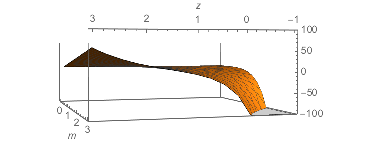
\includegraphics[scale = 0.8]{skewedlogit_before.png}
    \caption{F(z) for skewed logit model, z:[-1,3], m: [0.1,3]}
    \label{fig:skewedlogit_before}
\end{figure}

We will continue with 2 of \ref{proc} and add $e^z$ to the sequence.Through routine algebra, we have an equivalent sequence  \{$\Psi_0(z) = 1$, $\Psi_1(z) = z$,$\Psi_2(z) = z^2$,  $\Psi_3(z) = e^z$,$\Psi_4(z) = -(1+e^z)^2(-1+(1+e^{-z})^m)$\}. Here information matrix is expanded accordingly to  \[ \tilde{C}^*(\theta,z) = \phi(z)\left(\begin{array}{ccc}
-(1+e^z)^2(-1+(1+e^{-z})^m) &e^z&0\\
e^z&1 & z\\
0& z & z^2
\end{array} \right).\]

We then have $f_{1,1} = 1$, $f_{2,2} =2$, $f_{3,3} = e^z/2$, 
\begin{multline*}
     -f_{4,4} = e^{-z} \left(3 (m-1) m e^{-2 z} \left(2 e^z \left(e^z+1\right)+2 e^{2 z}\right) \left(e^{-z}+1\right)^{m-2}+3 m e^{-z} \left(2 e^z \left(e^z+1\right)+2 e^{2 z}\right) \left(e^{-z}+1\right)^{m-1}-4 m e^{-z} \left(2 e^z \left(e^z+1\right)+6 e^{2 z}\right) \left(e^{-z}+1\right)^{m-1}+\left(2 e^z \left(e^z+1\right)+14 e^{2 z}\right) \left(\left(e^{-z}+1\right)^m-1\right)+6 e^{2 z} \left((m-1) m e^{-2 z} \left(e^{-z}+1\right)^{m-2}+m e^{-z} \left(e^{-z}+1\right)^{m-1}\right)+6 e^z \left(e^z+1\right) \left((m-1) m e^{-2 z} \left(e^{-z}+1\right)^{m-2}+m e^{-z} \left(e^{-z}+1\right)^{m-1}\right)+\left(e^z+1\right)^2 \left((m-3) (m-2) (m-1) m e^{-4 z} \left(e^{-z}+1\right)^{m-4}+6 (m-2) (m-1) m e^{-3 z} \left(e^{-z}+1\right)^{m-3}+7 (m-1) m e^{-2 z} \left(e^{-z}+1\right)^{m-2}+m e^{-z} \left(e^{-z}+1\right)^{m-1}\right)+8 e^z \left(e^z+1\right) \left((m-2) (m-1) m \left(-e^{-3 z}\right) \left(e^{-z}+1\right)^{m-3}-3 (m-1) m e^{-2 z} \left(e^{-z}+1\right)^{m-2}-m e^{-z} \left(e^{-z}+1\right)^{m-1}\right)\right)\\-e^{-z} \left(-3 m e^{-z} \left(2 e^z \left(e^z+1\right)+2 e^{2 z}\right) \left(e^{-z}+1\right)^{m-1}+\left(2 e^z \left(e^z+1\right)+6 e^{2 z}\right) \left(\left(e^{-z}+1\right)^m-1\right)+6 e^z \left(e^z+1\right) \left((m-1) m e^{-2 z} \left(e^{-z}+1\right)^{m-2}+m e^{-z} \left(e^{-z}+1\right)^{m-1}\right)+\left(e^z+1\right)^2 \left((m-2) (m-1) m \left(-e^{-3 z}\right) \left(e^{-z}+1\right)^{m-3}-3 (m-1) m e^{-2 z} \left(e^{-z}+1\right)^{m-2}-m e^{-z} \left(e^{-z}+1\right)^{m-1}\right)\right)
\end{multline*}

     and $F(z)<0$ for $z\in (-\infty,\infty)$. We can also visually confirm through \ref{fig:skewedlogit_after} that the surface remains below $F(z)=0$ and thus the assumptions are confirmed. By our main result, it is known that there exist a complete class of 2 support points regardless of the model type. \begin{figure}[h]
    \centering
    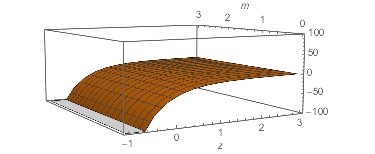
\includegraphics[scale = 0.8]{skewedlogit_after.png}
    \caption{$\tilde{F}(z)$ for skewed logit model, z:[-1,3], m: [0.1,3]}
    \label{fig:skewedlogit_after}
\end{figure}


\section{Conclusions}
Methods in Yang (2012) and Yang (2010) set up a unified strategy to find optimal design with minimal support for nonlinear models.  We extended its application to models that do not satisfy the assumptions and models defined on open intervals. The failed assumption is circumvented through adding ancillary terms in the function sequence, which may increase the number of support points needed. For certain types of models defined on open interval, the support may include the boundary points with 0 information and can be removed. A complete class of design with minimal support is then obtained. 
\bibliographystyle{plain}
\bibliography{bib_t} 
\end{document} 